\documentclass[journal,12pt,twocolumn]{IEEEtran}

\usepackage{graphicx}
\graphicspath{ {./5609/Assign4/} }

\makeatletter
\newcommand\xleftrightarrow[2][]{%
  \ext@arrow 9999{\longleftrightarrowfill@}{#1}{#2}}
\newcommand\longleftrightarrowfill@{%
  \arrowfill@\leftarrow\relbar\rightarrow}
\makeatother


\newcommand\leftarrowS{\leftarrow\joinrel\smalldollar}
\newcommand\rightarrowS{\smalldollar\joinrel\rightarrow}


\usepackage{amsmath}
\newcommand{\myvec}[1]{\ensuremath{\begin{pmatrix}#1\end{pmatrix}}}
\title{Assignment 4}
\author{PARIMISETTY HARINADHA (CS19RESCH11004)}
\begin{document}
\maketitle
\newpage
\begin{abstract}
This document presents the tracing of conic sections.
\end{abstract}
Download all python codes from 
\framebox[1\width]{ https://github.com/cs19resch11004/hari }
Download all Latex-tikz codes from 
\framebox[1.1\width]{ https://github.com/cs19resch11004/hari} 
\section{Problem}
Tracing of following equation
\begin{align}
    x^2+xy+y^2+x+y-1=0 \label{eq:1}
\end{align}
\section{solution}
The general equation of second degree is given by
\begin{align}
ax^2+2bxy+cy^2+2dx+2ey+f=0 
\end{align}

and can be expressed as
\begin{align}
\vec{x}^T V\vec{x}+2\vec{u}^T\vec{x}+f=0 \label{eq:3}
\end{align}
where
\begin{align}
V &= V^T = \myvec{a & b \\ b & c}\label{eq:4}
\\
\vec{u} &= \myvec{d \\ e}
\end{align}
Comparing equations \eqref{eq:1} and \eqref{eq:3} we get
\begin{align}
V=V^T&=\myvec{1 & \frac{1}{2} \\\\ \frac{1}{2} &1} \\
    \vec{u}&=\myvec{\frac{1}{2} \\\\\frac{1}{2} } \\
    f&=-1
\end{align}   

Expanding the Determinant of V.
\begin{align}
    \Delta_{V} &= \begin{array}{|cc|}
1 &\frac{1}{2}\\\frac{1}{2} & 1
\end{array}>0
\end{align}
Hence from above result, given equation represents the Ellipse.\\
The characteristic equation of V is obtained by evaluating the determinant 
\begin{align}
\begin{array}{|c|}
V-\lambda I
\end{array}&=0\\
\begin{array}{|cc|}
1-\lambda & \frac{1}{2} \\\\ \frac{1}{2} & 1-\lambda
\end{array}&=0
\end{align}
\begin{align}
(1-\lambda)(1-\lambda)-1/4=0\\
\lambda_{1}=\frac{1}{2},   \lambda_{2}=\frac{3}{2} \label{eq:13}
\end{align}
The eigenvector $\vec{p}$ is defined as 
\begin{align}
    V\vec{p}&=\lambda\vec{p}\\
    \implies (V-\lambda I)\vec{p}&=0 \label{eq:15}
\end{align}
For $\lambda_1=\frac{1}{2}$ ,
\begin{align}
    (V-\lambda_1I)=\myvec{\frac{1}{2} & \frac{1}{2} \\\\\frac{1}{2} & \frac{1}{2}}
\end{align}

 By row reduction,
\begin{align}
&\myvec{\frac{1}{2} & \frac{1}{2}\\ \\ \frac{1}{2} & \frac{1}{2}}
\xleftrightarrow[R_1\leftarrow 2R_1]{R_2\leftarrow 2R_2}
\myvec{1 & 1 \\ 1 & 1}
\end{align}

\begin{align}
&\xleftrightarrow{R_2\leftarrow R_2 - R_1}
\myvec{1 & 1 \\ 0 & 0 } \label{eq:18}
\end{align}

Subsituting equation \eqref{eq:18} in an equation \eqref{eq:15} we get
\begin{align}
        &   \myvec{1 & 1 \\ 0& 0}\myvec{u_1 \\ u_2}=\myvec{0 \\ 0}
\end{align}
Where, $\vec{p}=\myvec{u_1\\u_2}$
Let $u_1=t$
\begin{align}
    u_2&=-t
\end{align}


Eigen vector $\vec{p_1}$ is given by
\begin{align}
    \vec{p_1}&=\myvec{t \\ -t}
\end{align}
Let $t=1$, we get
\begin{align}
        \vec{p_1}&=\myvec{1 \\-1 } \label{eq:22}
\end{align}
For $\lambda_2=\frac{3}{2}$ ,
\begin{align}
(V-\lambda_2 I)&=\myvec{1-\frac{3}{2} & \frac{1}{2} \\\\\frac{1}{2} & 1-\frac{3}{2}}
&=\myvec{\frac{-1}{2} & \frac{1}{2} \\\\\frac{1}{2} & \frac{-1}{2}}
\end{align}

By row reduction,
\begin{align}
&\myvec{\frac{-1}{2} & \frac{1}{2}\\ \\ \frac{1}{2} & \frac{-1}{2}}
\xleftrightarrow[R_1\leftarrow 2R_1]{R_2\leftarrow 2R_2}
\myvec{-1 & 1 \\ 1 & -1}
\end{align}

\begin{align}
&\xleftrightarrow{R_2\leftarrow R_2 + R_1}
\myvec{-1 & 1 \\ 0 & 0 } \label{eq:25}
\end{align}

Subsituting equation \eqref{eq:25} in an equation \eqref{eq:15} we get
\begin{align}
        &   \myvec{-1 & 1 \\ 0& 0}\myvec{u_1 \\ u_2}=\myvec{0 \\ 0}
\end{align}
Where, $\vec{p}=\myvec{u_1\\u_2}$
Let $u_1=t$
\begin{align}
    u_2&=t
\end{align}


Eigen vector $\vec{p_2}$ is given by
\begin{align}
    \vec{p_2}&=\myvec{t \\ t}
\end{align}
Let $t=1$, we get
\begin{align}
        \vec{p_2}&=\myvec{1 \\1 }\label{eq:29}
\end{align}

By eigen decompostion V can be represented by
\begin{align}
    V&=PDP^T
\end{align}

where 
\begin{align}
P&=\myvec{\vec{p_1} & \vec{p_2}}\label{eq:31}\\
D&=\myvec{\lambda_1 & 0 \\0 & \lambda_2}\label{eq:32}
\end{align}

Substituting equations \eqref{eq:22}, \eqref{eq:29} in equation \eqref{eq:31} we get 
\begin{align}
    P&=\myvec{1 & 1 \\-1 & 1}
\end{align}
Substituting equation \eqref{eq:13} in \eqref{eq:32} we get
\begin{align}
       D&=\myvec{\frac{1}{2} & 0\\0 & \frac{3}{2}} \label{eq:34}
\end{align}

Centre of the ellipse is given by 
\begin{align}
    \vec{C}=-V^{-1}\vec{u}
\end{align}

\begin{align}
    \implies\vec{C}=-\myvec{\frac{4}{3}&\frac{-2}{3}\\\\\frac{-2}{3}&\frac{4}{3}}\myvec{\frac{1}{2}\\\\\frac{1}{2}}\\
    \implies\vec{C}=\myvec{\frac{-1}{3}\\\\\frac{-1}{3}}
\end{align}

Calculating the axes, we get
\begin{align}
a=\sqrt{\frac{\vec{u}^TV^{-1}\vec{u}-f}{\lambda_1}}=1.6329931618\\
b=\sqrt{\frac{\vec{u}^TV^{-1}\vec{u}-f}{\lambda_2}}=0.9428090416
\end{align}

Standard ellipse can be written in the form:
\begin{align}
    \vec{y}^TD\vec{y}=\vec{u}^TV^{-1}\vec{u}-f\label{eq:40}
\end{align}

Simplifying we get:
\begin{align}
\vec{u}^TV^{-1}\vec{u}=
\myvec{\frac{1}{2} &\frac{1}{2}}
\myvec{\frac{4}{3} & \frac{-2}{3}\\\frac{-2}{3} & \frac{4}{3}}
\myvec{\frac{1}{2}\\\frac{1}{2}} = \frac{1}{3}\label{eq:41}
\end{align}

Substituting equation \eqref{eq:41} in equation \eqref{eq:40}, then we have :
\begin{align}
 \vec{y}^TD\vec{y}=\frac{4}{3}  \label{eq:42}
\end{align}

Substituting  equation \eqref{eq:34}, in equation \eqref{eq:42} 
\begin{align}
    \vec{y}^T \myvec{\frac{1}{2} & 0\\0 &\frac{3}{2}}\vec{y}=\frac{4}{3}
\end{align}
\begin{align}
    \vec{y}^T \myvec{\frac{8}{3} & 0\\0 &\frac{8}{9}}\vec{y}=1
\end{align}
The following figure verifies the given equation \eqref{eq:3} as ellipse with centre $\myvec{\frac{-1}{3}\\\frac{-1}{3}}$
\begin{figure}[!ht]
\centering
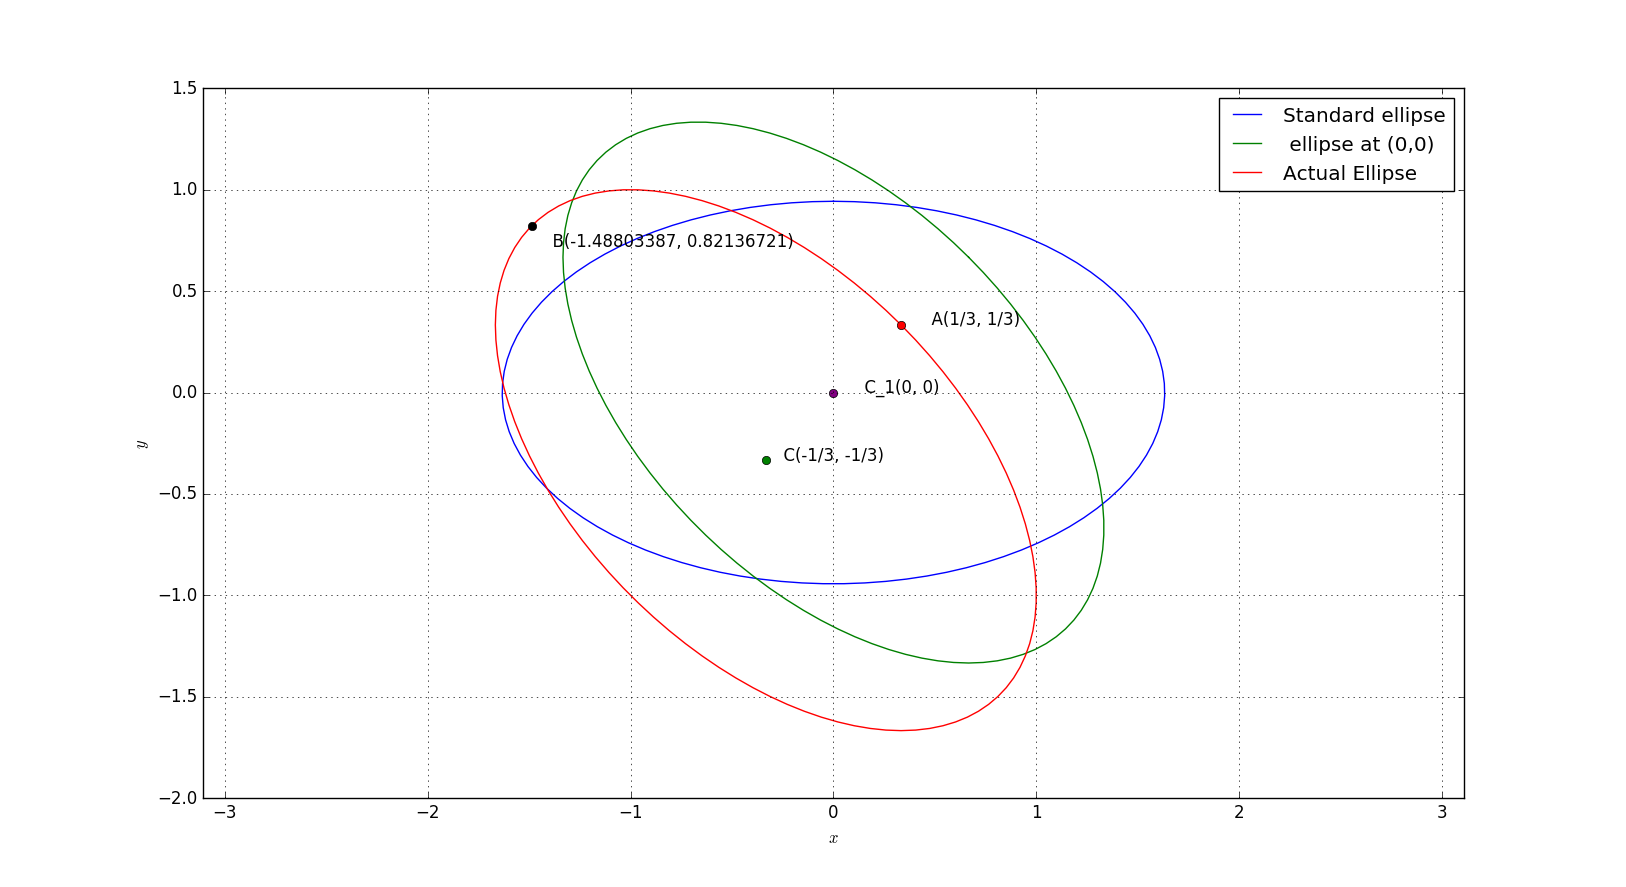
\includegraphics[width=\columnwidth]{fig.png}
\caption{Ellipse at C($\frac{-1}{3}$, $\frac{-1}{3}$), and Standard Ellipse}
\label{Fig}
\end{figure}

\end{document}
